\section{Theoretical Analysis}
\label{sec:analysis}

Firstly, we computed the central frequency and the gain depending on the frequency, utilizing the expressions from  the laboratory class.
We obtain the values of $1023.08 Hz$ for the central frequency, a bandwidth of $723.4 Hz$ and the following figure illustrates the gain:

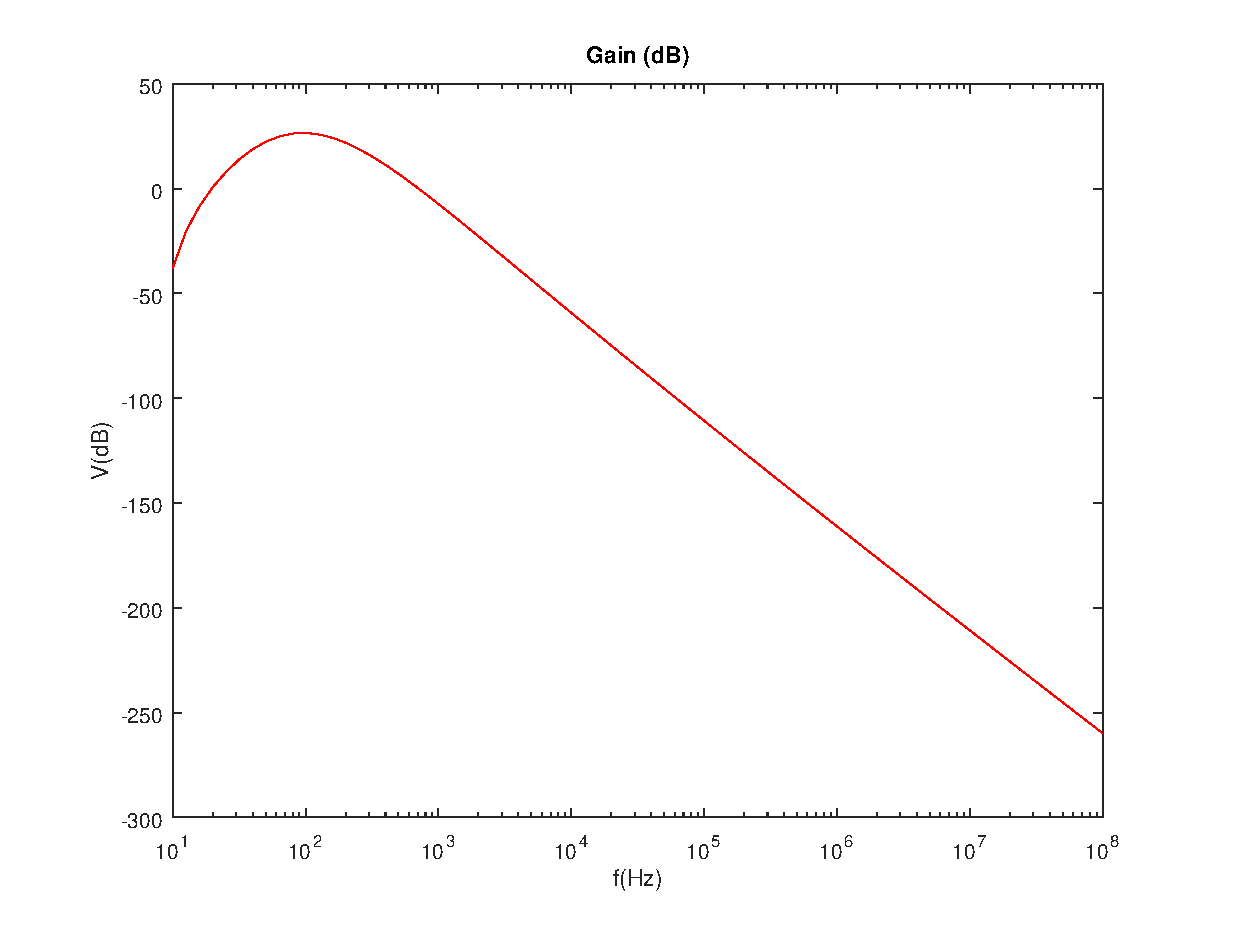
\includegraphics[width=0.8\linewidth]{teodB.eps}

We then used the incremental model of the OP-AMP component, yielding the following equations for the nodal analysis of the circuit:

A = [C1*w*i+1/R1+1/Zi,0,0,-1/Zi,0;
-Ao,1,0,Ao,0;
0,-1/Zo,1/R2+1/Zo+1/R3,-1/R3,-1/R2;
-1/Zi,0,-1/R3,1/R3+1/R4+1/Zi,0;
0,0,-1/R2,0,1/R2+C2*w*i]
    
B=[Vi*C1*w*i;0;0;0;0]

We therefore obtain the following plot for the gain as a function of frequency:

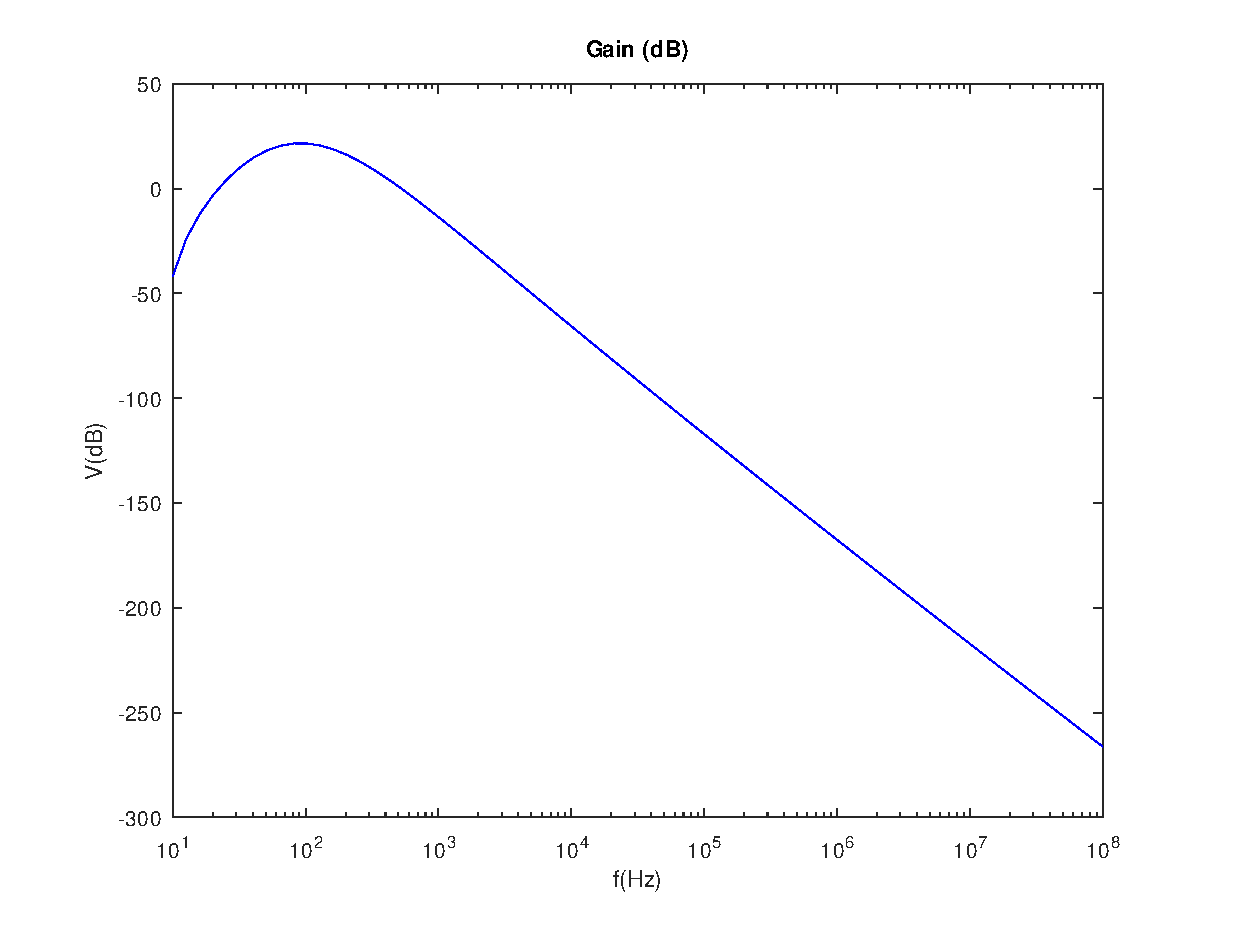
\includegraphics[width=0.8\linewidth]{t5dB.eps}

As such the central frequency is $ $, the gain at this frequency is $ $ and the bandwidth is $ $.

The input and output impedances were also calculated yielding values of $1009.6 Ohm$ and $2.24\cdot 10^{-5} Ohm$ respectively.